
\section{Risk Analysis}
An thorough analysis of possible risk scenarios was analysed and categorized. Both the probability and severity  of an event to occur is scaled from 1-10. Table \ref{probScale} and \ref{sevScale} shows the ranking system. The information given from this tables is feed into an risk assesment matrix. This matrix tells us how critical an risk is.

\begin {table}[h]
    \begin{minipage}{.5\linewidth}
        \begin{center}
        \caption {Probability scale} 
        \label{probScale} 
            \begin{tabular}{|c|c|}\hline 
            \rowcolor{cadetgrey}
            \textbf{Scale}   & \textbf{Probability(1-10)} \\ \hline 
            Low    &   1-3              \\ \rowcolor{gainsboro}
            Medium    &   4-7           \\
            High    &   8-10            \\ \rowcolor{gainsboro}
            \hline
            \end{tabular}
        \end{center}
    \end{minipage}
    \begin{minipage}{.5\linewidth}
        \begin{center}
        \caption {Severity scale} 
        \label{sevScale} 
            \begin{tabular}{|c|c|}\hline 
            \rowcolor{cadetgrey}
            \textbf{Scale}   & \textbf{Severity(1-10)} \\ \hline 
            Low   &   1-3               \\ \rowcolor{gainsboro}
            Medium    &   4-7           \\
            High    &   8-10            \\ \rowcolor{gainsboro}
            \hline
            \end{tabular}
        \end{center}
    \end{minipage}
\end{table}
%%%%%%%%%%%%%%%%%%%%%%%%%%%%%%%%%%%%%%%%%%%%%%%%%%%%%%%%%%%%%%%%
%%%%%%%%%%%%%%%%%%%%%%%%%%%%%%%%%%%%%%%%%%%%%%%%%%%%%%%%%%%%%%%%
\newpage
\subsection{Risk Assessment matrix}
The Risk assessment matrix shows us if we need to take care of an risk. If we multiply the probability with the severity  $P\cdot S$ we get the risk score.
\begin{figure}[h]
        \centering
            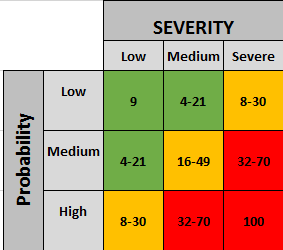
\includegraphics[width = 0.5\textwidth]{VAPIQ-PICTURES/RiskAssesMentMatrix.png}
            \caption{PICTURE caption}
            \label{fig:testpic2}
        \hfill
\end{figure}